\chapter{Einleitung} \label{Einleitung}

%Kurze Erläuterung der Aufgabenstellung und der Messmethode, d.h. stichwortartige 
%Zusammenstellung von wesentlichen Definitionen, Formeln, etc. (keine Herleitungen, 
%keine seitenlange Darstellung von Lehrbuchwissen!). 


\begin{figure}[h]
    \centering
    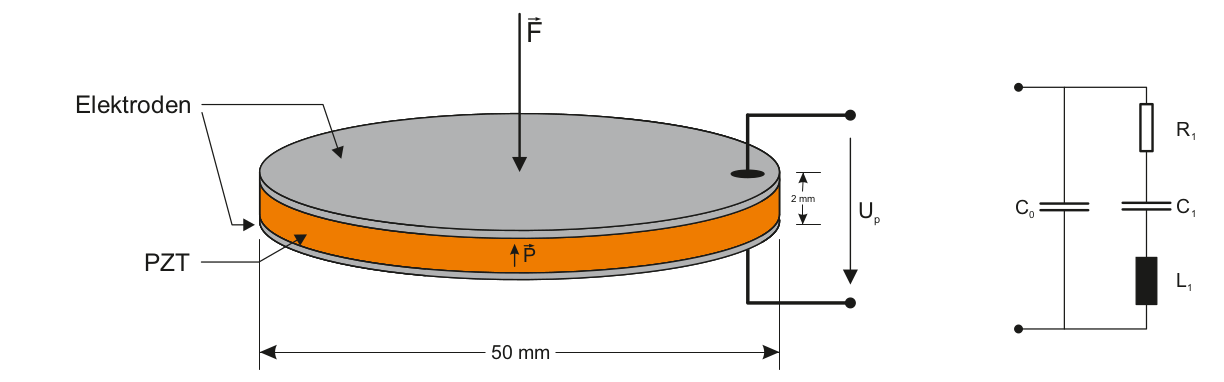
\includegraphics[width=1 \textwidth]{image/Piezo_Skizze.png}
    \caption{Piezoelektrische Scheibe mit Ersatzschaltbild  \cite{laborpraktikum2022} }
\end{figure}

\section{Vorbereitung}

Piezomaterial können grundsätzlich in harten und weichem Material unterteilt werden. 
Feroelektrisch weiche Materialien lassen sich im Vergleich leicht Polarisieren. Damit weißen diese einen hohen Kopplungsfaktor, sowie hoher Defomationskonstante. \\
Der Kopplungsfaktor für den Pz27 in Dickenrichtung beträgt 0.70 . \\





\begin{figure}
    \centering
    \includesvg[width=1 \textwidth]{Berechnungen/Impedanzgang}
    \caption{theoretischer Impedanzgang}
\end{figure}